\subsection{Hardware used}

For the construction of our robot we were given the following components, not all of them were used in the final construction:
\begin{itemize}
\item Roboard (Roboard-100)
\item Serializer board
\item Custom made powerboard
\item 2 motors with encoders
\item 2 wheels for each side
\item 1 caster wheels
\item Aluminum plates
\item Sonar (Devantech SRF08)
\item 1 web cameras (Logitech C905)
\item 6 short range, 2 long range IR-sensors (Sharp GP2D120XJ00F/GP2D12J0000F)
\item Wireless USB Adapter (Belkin P-F5D8053)
\item Battery(LiPo) with charger(team Orion advantage IQ605)
\item Lots of wires and other stuff that was needed to mount everything
\end{itemize}


\subsection{Mechanical Design}

Before start designing and building the robot, there were some constraints to consider:
\begin{itemize}
\item The robot can not be wider than 40 cm and it can not be taller than 29 cm.
\item It must be fairly circular to avoid hitting obstacles when rotating.
\item The camera must be placed in such way that it can detect tags that are placed at least 10 cm and at most 25 cm from the floor.
\item The IR-sensors must be fitted inside the error threshold.
\end{itemize}
Besides the constraints above, we decided to not build everything at once but to build the basics in such way that we can easily add and make changes to it. This resulted in several changes for the placement of the sensors.
The basic design was also drawn in a 3D modelling program (Google Sketchup) to test different configuration before actually putting them together.

\begin{figure}[h!]
\label{fig:google_sketchup_draw1}
    \begin{centering}
   	 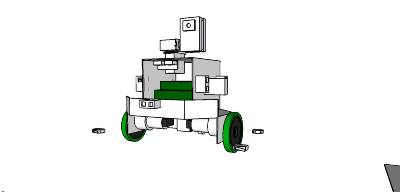
\includegraphics[scale=1.0]{figures/g_sketchup_v7.jpeg}
   	 \caption{The final 3D model version in Google Sketchup}\label{fig:google_sketchup_draw1}
    \end{centering}
\end{figure}


\begin{figure}[h!]
\label{fig:amee_final}
    \begin{centering}
   	 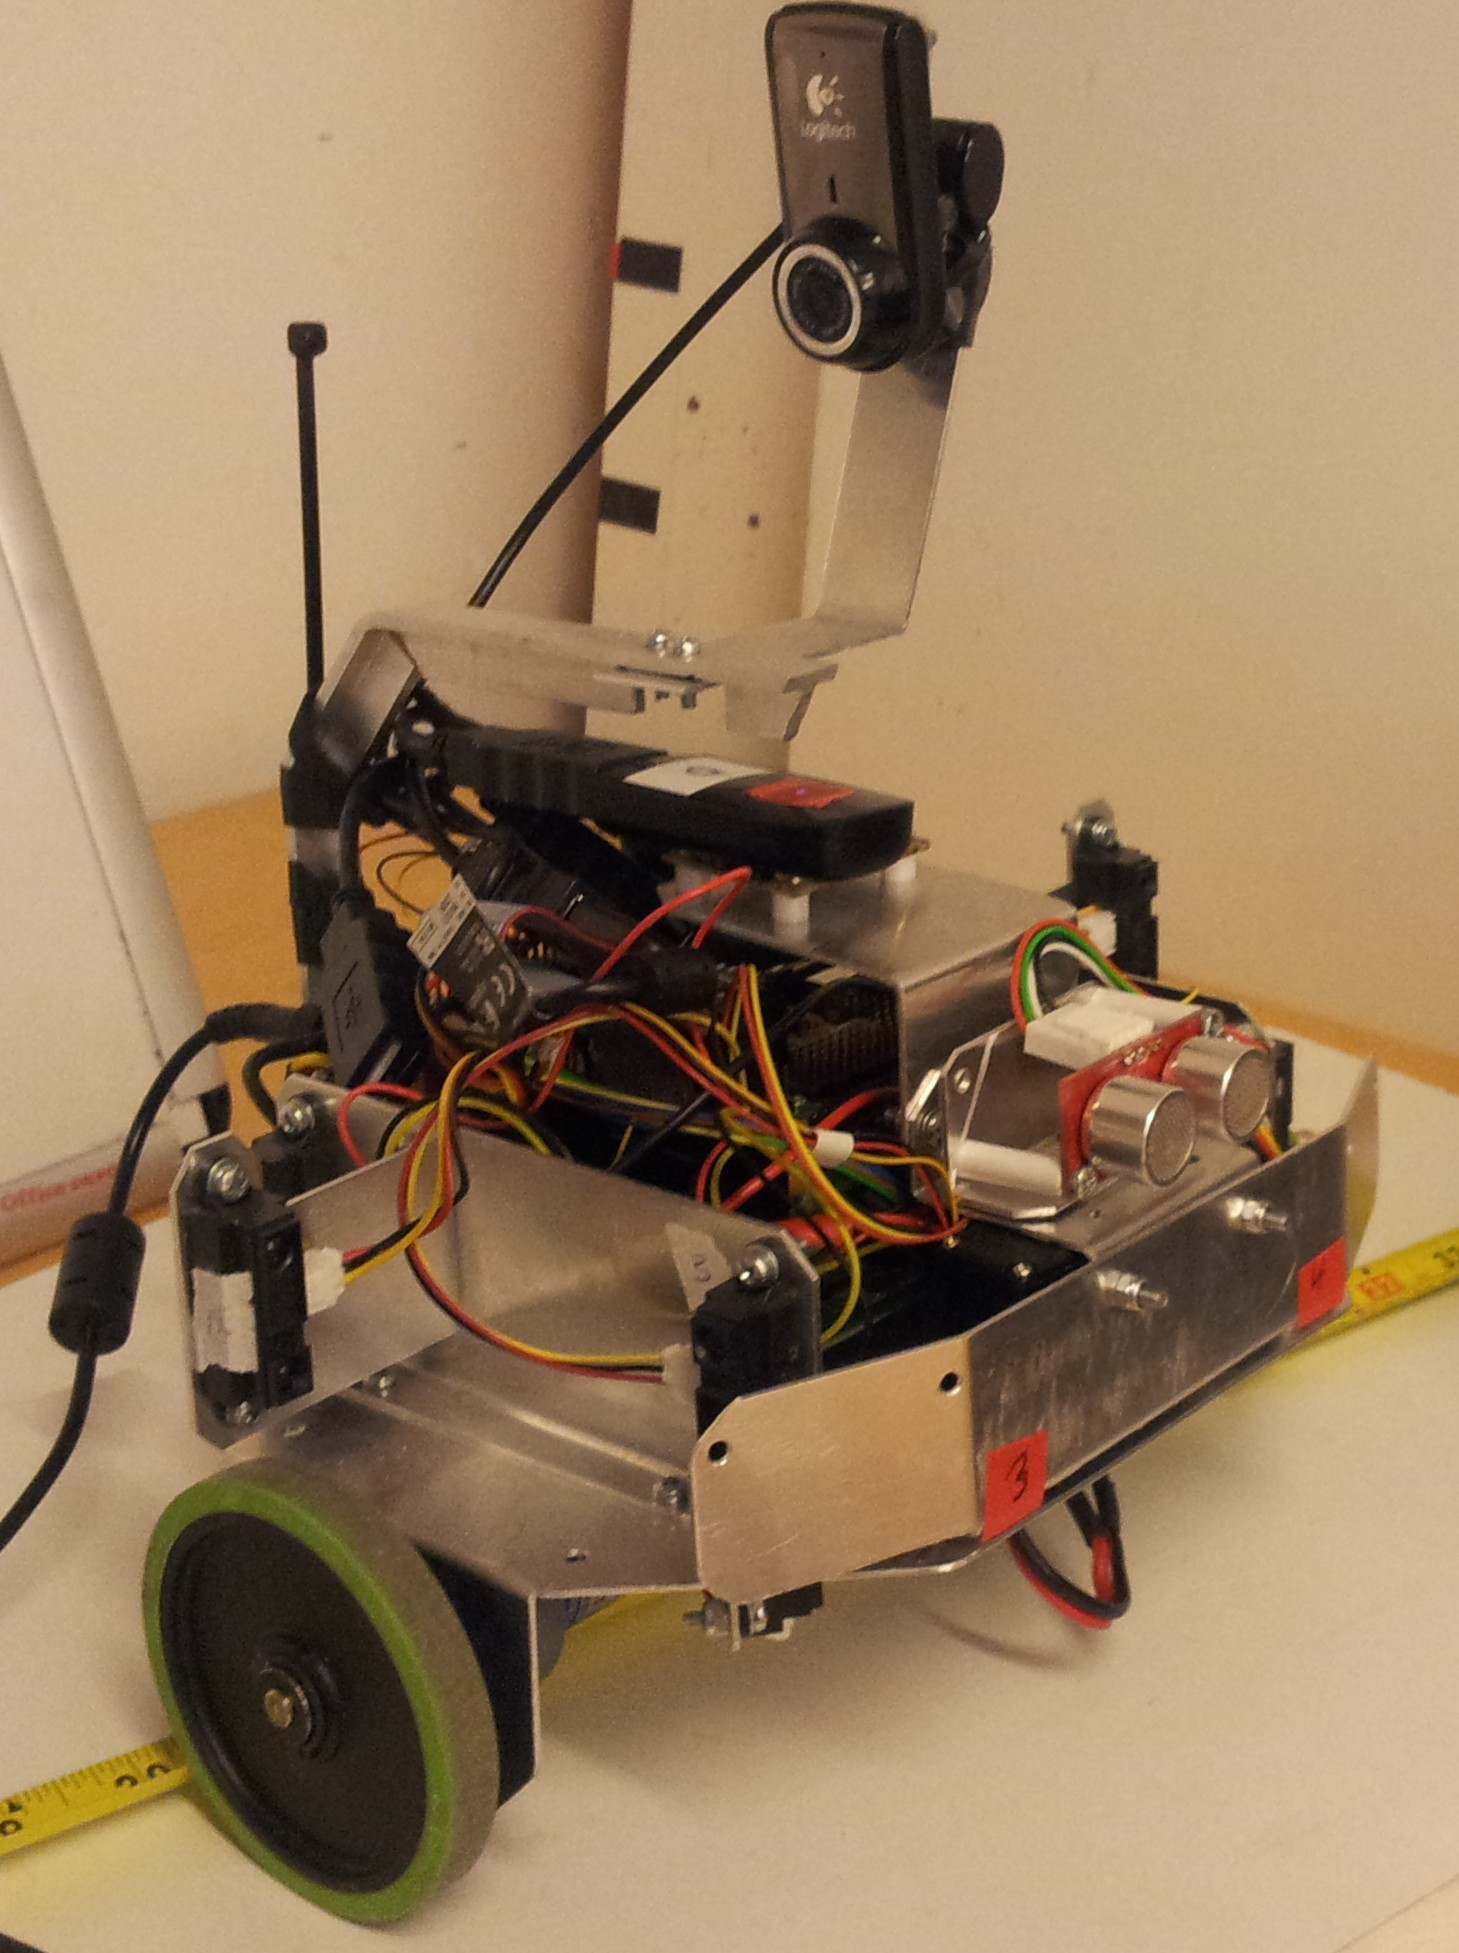
\includegraphics[scale=0.1]{figures/amee_final.jpg}
   	 \caption{The final hardware design}\label{fig:amee_final}
    \end{centering}
\end{figure}

\subsection{Sensors}

Sensors are used to tell the robot what happens in it's surrounding or how it has moved. 
In order to achieve a proper movement control, sensor feedback is required so that the controlling unit can know what the actuators actually do with the control signal. There is a delay in the actuation, since motors doesn't react instantly on a voltage applied to it, and also some uncertainty. This robot make use of 3 different types of sensors to sense the environment and localize itself. The sensors are listed and explained below:
\begin{itemize}
\item Wheel encoders outputs tics where each tic corresponds to a certain rotation of the motor axis. The tics are converted to a distance so that the movement can be determined. The movement is integrated over time so that a position and heading is obtained with respect to the starting position and heading. However, the odometry is not perfect since the wheels slip when the robot turns, accelerates and brakes. 

\item IR sensor outputs a voltage that is based on the reflected intensity of the reflected light. This voltage is then read by the robot's analog to digital converter and the voltage is translated into a distance. This measurement doesn't have any drift since the measurement is relative to a wall and not something that is integrated over time. However the downside is that the reflections can be misleading if it reflects from an edge or a different material. It is also limited in the measuring range.

\item Sonar sensor which measures the distance to the closest obstacle in front of it. This could be used for detecting small obstacles in front of the robot since it sees an area in front of the robot and not just in a line as the IR sensors do.

\item A fourth sensor is a camera and is used for finding and classifying tags. This is further described in section \ref{sect:computerVision}.

\end{itemize}